\section{Eigenvalue problem of the Landau levels of a Weyl Hamiltonian}
To evaluate the correlator of the response function, the matrix elements of the current and stress-energy tensor must be found.
In order to do this, we find eigenstates in the Landau basis of the system.
We will first consider the untilted Hamiltonian, which we will then use to find the Landau levels of the tilted Hamiltonian.

\subsection{The untilted Hamiltonian}
The Weyl Hamiltonian
\begin{equation}
  \label{eq:weyl-hamil}
  H_s = s v_F \sigma^i \left( p_i + e A_i \right),
\end{equation}
with $s$ being the chirality, $p_i$ the momentum operator, and $e = |e|$ the coupling constant to the electromagnetic field $\vec{A}$.
Choose coordinates such that $\vec{B} = B_z \hat{\vec{z}}$, which in the Landau gauge gives $\vec{A} = -B_{z}y \: \hat{\vec{x}}$.
As the Hamiltonian is invariant in $x$ and $z$, take the plane wave ansatz $\phi(\vec{r}) = e^{ik_x x + i k_z z} \phi (y)$.
It then follows
\begin{equation}
  H_s \phi(\vec{r}) = E \phi(\vec{r}) \implies \tilde{H}_s \phi(y)  = E \phi(y),
\end{equation}
where $\tilde{H}$ is the result of replacing $p_z \to \hbar k_z, p_x\to \hbar  k_x$ in $H_s$, as the plane wave part of $\phi $ have these eigenvalues.
Absorb the chirality $s$ as a sign in the velocity $v_F$, for more concise notation.
Thus, writing everything explicitly, the spectrum is given by
\begin{equation}
  \label{eq:15}
  -\hbar  v_F
  \begin{pmatrix}
    - k_z & \partial _y + e y B_{z} / \hbar  - k_x\\
    -\partial _y + e y B_{z} / \hbar -k_x & k_z
  \end{pmatrix}
  \phi(y)  = E\phi(y).
\end{equation}
We will now find the spectrum $E$ of the Hamiltonian.

Inspired by the derivation for the spectrum of the 2D Dirac Hamiltonian in~\cite{wehlingDiracMaterials2014}, we introduce the length scale $l_B = \sqrt{\hbar / eB}$, and the dimensionless quantity $\chi = y /l_{B} - k_x l_{B}$.
In dimensionless quantities Eq. (\ref{eq:15}) becomes
\begin{equation}
  -\frac{{\hbar v_F}}{l_{B}}
  \begin{pmatrix}
    -k_z l_B & \partial _{\chi } + \chi \\
    -\partial _{\chi } + \chi & k_z l_B
  \end{pmatrix}
  \phi(y)  =  E \phi(y).
\end{equation}
Let the operators \(a = \left( \chi + \partial _{\chi } \right) / \sqrt{2},\; a^{\dagger} = \left( \chi - \partial _{\chi } \right) /\sqrt{2}\).
One may easily verify the commutation relation $[a, a^{\dagger}] = 1$;
they are ladder operators of the harmonic oscillators, whose eigenstates are $\ket{n}$, and where $a\ket{n} = \sqrt{n}\ket{n-1}, a^{\dagger} \ket{n} = \sqrt{n+1} \ket{n+1}$.
In terms of these operators, the system is
\begin{equation}
  -\frac{\sqrt{2} \hbar v_F}{l_B}
  \begin{pmatrix}
    -\frac{k_zl_B}{\sqrt{2}} & a\\
    a^{\dagger} & \frac{k_zl_B}{\sqrt{2}}
  \end{pmatrix}
  \ket{\phi } = E \ket{\phi }.
\end{equation}
Take the ansatz
\begin{equation}
  \ket{\phi } =
  \begin{pmatrix}
    \beta \ket{n-1}\\
    \alpha  \ket{n}
  \end{pmatrix},
\end{equation}
which is the most general form of $\ket{\phi }$ with any hope of being an eigenstate.
This leads to
\begin{equation}
  -\frac{\sqrt{2} \hbar v_F}{l_B}
  \begin{pmatrix}
    \left( -\gamma \beta + \alpha \sqrt{n} \right) \ket{n-1}\\
    \left( \beta \sqrt{n} + \gamma \alpha \right) \ket{n}
  \end{pmatrix}
  = E \ket{\phi },
\end{equation}
with $\gamma  = k_zl_B / \sqrt{2}$.
For $n > 0$ this leads to the equation for $\phi $ to be an energy eigenfunction
\begin{equation}
  -\gamma + \frac{\alpha}{\beta } \sqrt{n} = \frac{\beta }{\alpha } \sqrt{n} + \gamma.
\end{equation}
Solving for $\alpha /\beta $ this gives
\begin{equation}
  \frac{\alpha}{\beta } = \frac{\gamma}{\sqrt{n}} \pm \sqrt{1 + \frac{\gamma^2}{n}},
\end{equation}
and thus
\begin{equation}
  E = \pm v_F \sqrt{
    \frac{2n \hbar ^2}{l_B^2} + k_z^2\hbar ^2
  }
  = \pm s v_F \sqrt{
    2n e B \hbar + k_z^2\hbar ^2
  },
\end{equation}
where we reintroduced the explicit $s$.
For $n = 0$ the annihilation operator $a$ destroys the vacuum state $\ket{0}$, and the energy is instead $E_0 = -\hbar s k_z v_F$.
The excited energy states are doubly degenerate;
we choose to denote the energy levels by $m \in \mathbb{Z}$, where the sign from $\pm s$ is taken care of by the sign of this quantum number, and the harmonic oscillator levels $n$ are given by its absolute value $|m|$.
The energy levels are
\begin{align}
  E_{k_z m s} &= \operatorname{sign}(m) v_F \sqrt{2 |m| e B \hbar  + k_z^2 \hbar ^2} & \text{ for } m \neq 0,\\
E_{k_z 0 s} &= -s \hbar k_z v_F & \text{ for } m = 0.
\end{align}

We now find the corresponding eigenvectors of the system.
The solution to the one dimensional harmonic oscillator in position space is, in dimensionless coordinates $\xi$,~\cite[Eq.~18.39.5]{NIST:DLMF}
\begin{equation}
  \braket{\xi | n} = \phi _n (\xi)
  = \frac{1}{\sqrt{2^nn!}} \pi^{-\frac{1}{4}}
  e^{- \frac{\xi^2}{2}} H_n \left( \xi \right),
  % = \frac{1}{\sqrt{2^nn!}} \left( m\frac{\omega}{\pi \hbar } \right)^{\frac{1}{4}}
  % e^{- \frac{{m\omega x^2}}{2\hbar }} H_n \left( \sqrt{\frac{m\omega }{\hbar } x} \right),
\end{equation}
where $H_n$ are the Hermite polynomials.
Thus,
\begin{equation}
  \braket{\chi | \phi } =
  \begin{pmatrix}
    \beta \braket{\chi | n-1}\\
    \alpha \braket{\chi | n}
  \end{pmatrix}
  =
  e^{- \frac{\chi^2}{2}}
  \begin{pmatrix}
    \frac{\beta }{\sqrt{2^{n-1}(n-1)!\sqrt{\pi }}} H_{n-1} \left( \chi \right)\\
    \frac{\alpha }{\sqrt{2^{n}n!\sqrt{\pi }}} H_n \left(\chi \right)\\
  \end{pmatrix}
\end{equation}
Choosing
\begin{equation}
  \alpha  = \sqrt{\frac{\gamma^2}{n}} \implies \beta = \frac{1}{1 \pm \sqrt{1 + \frac{n}{\gamma ^2}}} = \pm \frac{\gamma ^2}{n} \left( \sqrt{1 + \frac{n}{\gamma ^2}} - 1 \right),
\end{equation}
gives
\begin{equation}
  \phi (\chi ) = e^{-\frac{\chi^2}{2}} \sqrt{\frac{\gamma ^2}{n}}
  \begin{pmatrix}
    \frac{
      \pm \sqrt{\frac{\gamma ^2}{n}} \left( \sqrt{1 + \frac{n}{\gamma ^2}} - 1 \right)
    }{
      \sqrt{2^{n-1} (n-1)! \sqrt{\pi }}
    }
    H_{n-1}(\chi )\\
    \frac{1}{\sqrt{2^{n}n!\sqrt{\pi }}} H_n \left(\chi \right)
  \end{pmatrix}.
\end{equation}
There are thus four quantum numbers related to the eigenvectors, $k_x,  k_z, m, s$.
Reintroducing $\chi = (y-k_xl_B^2) /l_B$ and normalizing
\begin{equation}
  \phi _{\vec{k} m s}(\vec{r}) = \frac{1}{\sqrt{L_xL_z}}
  \frac{e^{ik_x x}e^{ik_z z}}{\sqrt{\alpha_{k_z m s}^2 + 1}}
  e^{-\frac{\left(y-k_x l^2\right)^2}{2 l_B^2}}
  \begin{pmatrix}
    \frac{\alpha_{k_z m s}}{\sqrt{2^{M-1} (M-1)! \sqrt{\pi } l_B}} H_{M-1}\left( \frac{y-k_x l_B^2}{l_B} \right)\\
    \frac{1}{\sqrt{2^M M! \sqrt{\pi } l_B}} H_M \left( \frac{y-k_x l_B^2}{l_B} \right)
  \end{pmatrix},
\end{equation}
where capital letters indicate absolute value of corresponding quantity, $M=|m|, \vec{k} = (k_x, k_z)$, and with the normalization factor
\begin{equation}
  \alpha_{k_z m s} = \frac{-\sqrt{2eB\hbar M}}{\frac{E_{k_z m s}}{s v_{F}} - \hbar  k_z}.
\end{equation}

\subsection{The tilted Hamiltonian}
\todo{Consider which formalism to use for this section. Should we already here use the geometry, or keep it with parallell, perpendicular?}
\todo{I think it is better to use perp, parallell here, and then transition to using the explicit geometry later}

The eigenvalues of Type-II Weyl semimetal are simple to find, and are not qualitatively different from those of Type-I, other than the appearance of particle and hole pockets at the Fermi level.
We will also consider the Landau levels of these materials, which importantly are very different from Type-I.
In fact, erroneous treatment of the Landau spectrum of Type-II semimetals caused the original paper describing Type-II materials to mistakenly assert that the chiral anomaly would not be present for certain directions of a background magnetic field \cite{soluyanovTypeIIWeylSemimetals2015}\cite{sharmaChiralAnomalyLongitudinal2017}.

Eigenstates, spin, berry, etc

The issue with the Landau level description is that for certain directions of the \(B\)-field, the Landau levels break down.
For Type-I materials, the description is valid for all directions of the \(B\)-field, but as the cone tip into a Type-II material, the description breaks down when the \(B\)-field and tilt direction are perpendicular \cite{sharmaChiralAnomalyLongitudinal2017}, and as the magnitude of the tilt increases, the Landau levels are only valid up to a certain angle between the tilt direction and magnetic field.
We will in this section derive and elucidate the Landau levels and their regions of validity.

Consider the Hamiltonian
\begin{equation}
  \label{eq:16}
  H = v_{F} \vec{t}^s  \vec{k} + s v_{F} \vec{k} \vec{\sigma},
\end{equation}
where \(\vec{t}^s\) is the \emph{tilt vector} and \( v_F \) is the Fermi velocity
\footnote{In general, the Fermi velocity may be anisotropic, in which case the momentum enter as \( v_i k_i \), instead of \( v_F k_i \). By a rescaling of the momenta, we may consider any, in general anisotropic, system to be isotropic in velocity.}.
To find the Landau levels in a magnetic field \(\vec{B} = B_{z}\hat{z} \), we will ``Lorentz boost'' the system to a frame where the cone is not tilted, where we may use the usual approach for finding the Landau levels.
Firstly, assume that the tilt vector \(\vec{ t }\) is in the \(x,z\)-plane, \(\vec{t} = (t_{\perp}, 0, t_{\parallel})\), which we can always achieve by a rotation around \(z\).
\todo{Proof by figure}
Introduce the \(\vec{B}\)-field by the minimal coupling \(\vec{k} \to \vec{k}^B = \vec{k} + e \vec{A}\).
We take the field to be in the \( z \)-direction, and use the Landau gague \(\vec{A} = -B_{z}y \hat{x}\).

The Landau level equation is
\begin{equation}
  \label{eq:17}
  \left(H_{B} - E\right) \ket{\psi } = 0,
\end{equation}
with
\begin{equation}
  \label{eq:18}
  H_{B} = v_F \left(t^s _{\perp} k^B_{x} + t^s _{\parallel} k^B_{z} \right) \mathcal{I}_2 + \sum_i s v_{F} k^B_{i} \sigma _{i},
\end{equation}
where \(\mathcal{I}_{2}\) is the identity matrix of size 2.
In order to use the ladder operator method used for the untilted cone, we must get rid of the \(k^B_{x}\) on the diagonal of the Hamiltonian.
\footnote{It would also be possible to choose the frame such that the tilt was both in \(x\) and \(y\) direction, in which case we would get ladder operators also on the diagonal.
  This system, albeight tedious, could also have been solved directly.
  \todo{Verify this}
}
To achieve this, we will use a ``Lorentz transformation'', which as we will show only leave \(k_{z}\) and \(E\) in the diagonal.
Act with the hyperbolic rotation operator \(R = \exp[\Theta /2 \sigma_{x}]\) on Eq. \eqref{eq:17}, and insert identity on the form \(\exp[\Theta /2 \sigma_{x}]\exp[-\Theta /2 \sigma_{x}]\) before the state vector.
By introducing the state in the rotated frame \(\ket{\tilde{\psi}} = \exp[- \Theta /2 \sigma_{x}] \mathcal{N} \ket{\psi } \), with \(\mathcal{N}\) a normalization factor compensating for the non-unitarity of the transformation, we get the eigenvalue equation
\begin{equation}
  \label{eq:19}
  (\exp[\Theta /2 \sigma_{x}] H_{B}\exp[\Theta /2 \sigma_{x}] - E \exp[\Theta \sigma_{x}]) \ket{\tilde{\psi}} = 0.
\end{equation}

We now make the fortunate observation that the diagonal elements of
\[
  R \sigma_{i} R
\]
are zero for $i=y$ and non-zero for \(i=x,z\).
We may thus rotate the \(x\) and \(z\) in and out of the diagonal elements, without accidentaly rotating the \(y\) components into the diagonal.

The problematic part of the Hamiltonian with regards to finding the Landau levels, are the terms containing \(k^B_{x}\) on the diagonal, i.e.
\[
  v_F t^s_{\perp} k^B_{x} \mathcal{I}_{2} + s v_{F} k^B_{x} \sigma _{x}.
\]
We will now find the boost parameter that eliminates \(k_{x}\) from the diagonal.
We have
\begin{equation}
  \label{eq:20}
  R^{2} = e^{\Theta \sigma _{x} } =
  \begin{pmatrix}
    \cosh \theta & \sinh \theta \\
    \sinh \theta & \cosh \theta
  \end{pmatrix}
\end{equation}
and as $[R, \sigma_{x}] = 0$,
\begin{equation}
  \label{eq:21}
  R \sigma _{x} R =  R^{2} \sigma _{x} =
  \begin{pmatrix}
    \sinh \theta & \cosh \theta \\
    \cosh \theta & \sinh \theta
  \end{pmatrix},
\end{equation}
as the effect of \(\sigma _{x}\) is to transpose the rows.
The requirement for \(k^B_{x}\) to be rotated out of the diagonal is thus
\begin{equation}
  \label{eq:22}
  t^s_{\perp} \cosh \theta + s \sinh \theta = 0.
\end{equation}
Solving for \(\theta \) we get
\begin{equation}
  \label{eq:23}
  \theta = \log (
  \pm \frac{\sqrt{s - t^s_{\perp}}}{\sqrt{s + t^s_{\perp}}}
  ).
\end{equation}
\todo{NB: depending of choice of sign in log, we get different signs in answer}
Alternatively, written in a slightly suggestive form,
\begin{equation}
  \label{eq:24}
  \tanh \theta =
  - s t^s_{\perp}.
\end{equation}
\todo{For pedagogic reasons, include arctanh, which is only valid for -1 < x < 1, explicitly showing the collapse?}

Expressed in the parameter \(t\), the result in Eq. \eqref{eq:24} has an intuitive, and quite visual, interpretation.
As described above, we have rotated our frame such that the tilt is confined to the \(x,z\)-plane, i.e. no tilt in the \(y\)-direction.
The required hyperbolic tilt angle to eliminate the \(k^B_{x}\) in the diagonal elements of the Hamiltonian, originating from the tilt, was
\begin{equation}
  \label{eq:25}
  \theta = - s \tanh^{-1} t^s_{x}.
\end{equation}
The inverse of \(\tan \), of course, diverges as the argument approaches \(\pm 1\), as shown in Figure \ref{fig:arctanh}.
\begin{figure}[ht]
  \tikzsetnextfilename{arctanh}
  \centering
  \begin{tikzpicture}
    \pgfkeys{/pgf/declare function={arctanh(\x) = 0.5*(ln((1+\x)/(1-\x)));}}
    \begin{axis}[
      xmin=-1.2, xmax=1.2,
      ymin=-3.9, ymax=3.9,
      samples=200,
      enlarge x limits=false,
      grid=both,
      no markers,
      % axis equal
      xlabel=\(x\),
      ylabel=\(\tanh^{-1} x\),
      % ytick=none,
      ]
      \addplot +[thick,domain=-0.999:0.999] {arctanh(x)};
      \draw [thick,dashed,domain=-0.99:0.99] (1,-4) -- (1,4);
      \draw [thick,dashed,domain=-0.99:0.99] (-1,-4) -- (-1,4);
    \end{axis}
  \end{tikzpicture}
  \caption{\label{fig:arctanh} Plot of \(\tanh^{-1}\), which diverges as the argument goes to \(\pm 1\).}
\end{figure}
For \(|t_{x}| < 1\) we are able to find an angle \(\theta \) which transforms our Hamiltonian into a form which we may solve.
For \(|t_{x}| \geq 1\), however, no (real) solution of \(\theta \) exits, and the Landau level description collapses.
More concretely, as we will show later, the separation of the landau levels is reduced as the perpendicular tilt increases, and as \( |t_x| \to 1 \), the level separation \( \Delta E \to 0 \).

\todo{ Discuss magnetic vs electric regime }


Interestingly, there are no restrictions in the perpendicual tilt, \( t_z \).
The \( \vec{t} \) parametrization of the tilt is conveniently visualized by plottin the \( t \)-vector inside a unit sphere, shown in Figure \ref{fig:tiltSphere}.
If the vector is outside the unit sphere, it is a Type-II, if it is inside, it is a Type-I.
Also, if the projection of the vector onto the \(x,y\)-plane is on the unit disk, the Landau level description is valid, if not, the Landau levels collapse.
All Type-I materials may thus be described by Landau levels, while it for Type-II is only valid for certain directions of the \(t\)-vector.
As the \(t\)-vector gets larger, the region of valid directions is reduced to an ever smaller cone around \(z\).
\begin{figure}[ht]
  \centering
  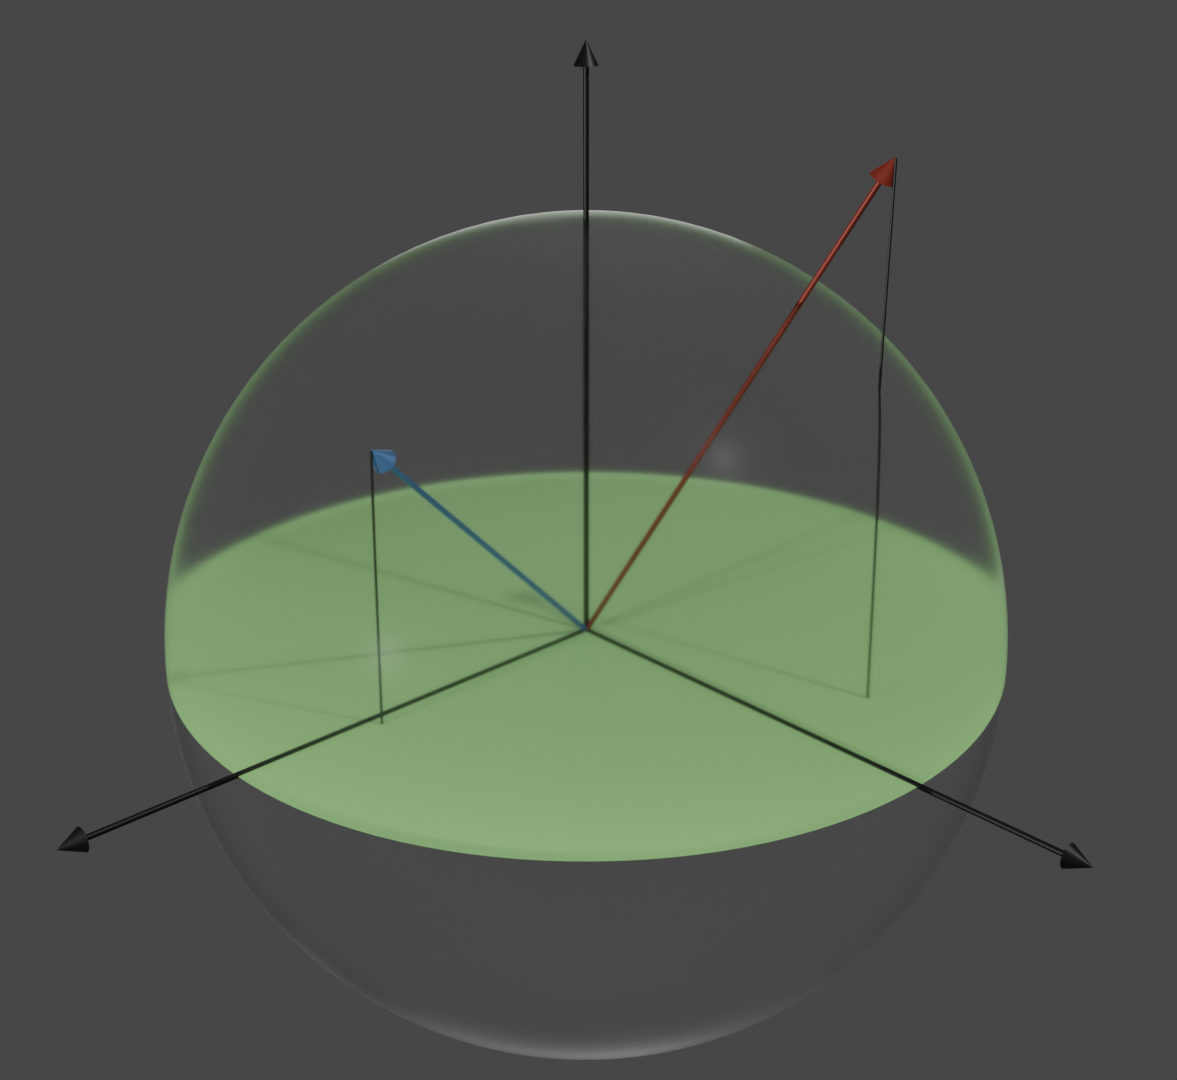
\includegraphics[width=0.75\textwidth]{figures/tiltSpherewBackground.png}
  \caption{\label{fig:tiltSphere} TODO}
\end{figure}

We now return to solving Eq.~\eqref{eq:19}, using the solution angle we just found.
By insertion, and after some clean up, we get
\emph{note to thorvald: we chose \(\theta = Log \left(+ \dots\right) \)}
\begin{multline}
  \label{eq:26}
  (\exp[\Theta /2 \sigma_{x}] H_{B}\exp[\Theta /2 \sigma_{x}] - E \exp[\Theta \sigma_{x}]) \ket{\tilde{\psi}} = 0\\
  = v_F \begin{pmatrix}
          k_z ( s + t^s_z \gamma ) - E / v_F \gamma & -s ( ik_y + k_z t^s_x t^s_z \gamma - k_x / \gamma - E /v_{F} \gamma t^s_x)\\
          s ( i k_y - k_z t^s_x t^s_z \gamma + k_x / \gamma + E /v_F \gamma t^s_x) & - k_z (s - t^s_z \gamma) - E \gamma
        \end{pmatrix}\\
    \ket{\psi}.
\end{multline}
In order to simplify this further, absorb \(\gamma t^s_x (k_{z} t^s_{\parallel} - E /v_{F}) \) into \(k_{x}\).
Thus, let
\begin{equation}
  \label{eq:27}
  \begin{split}
    \tilde{k}_{x} &= k_{x} / \gamma + \gamma t^s_x ( E /v_F - k_{z} t^s_{\parallel}),\\
    \tilde{k}_{y} &=  k_{y},\\
    \tilde{k}_{z} &=  k_{z}.\\
  \end{split}
\end{equation}

These expressions warrant some explanation, as the Lorentz boost is of course
\begin{equation}
  \label{eq:28}
  \tilde{k}_x = \gamma (k_x - \beta \frac{E}{v_{F}}),
\end{equation}
\todo{comment on beta = tx, or change to tx}
where we used the four momentum \( p^{\mu } = (\frac{E}{v_{F}}, \vec{p}) \), and the effective speed of light \( v_F \).
It can thus look like our expression in Eq. \eqref{eq:27} is wrong.
The solution to this seeming inconsitency is that the proper energy is not \( \frac{E}{v_{F}} - k_z t_{\parallel} \), but rather \( \frac{E}{v_{F}} - k_z t_{\parallel} - k_x t_{\perp}\).
\todo{Something smart here}

The eigenvalue equation is simply
\begin{equation}
  \label{eq:29}
  \left[  \gamma \left( t^s_{\parallel} \tilde{k}_{z} - \frac{E}{v_{F}} \right) \mathcal{I}_{2} +
  s \tilde{k}_{i} \sigma _{i} \right] \ket{\tilde{\psi}}= 0.
\end{equation}
If we now again introduce the magnetic field using minimal coupling, \(k_{x} \to  k_{x} - ey B_{z} \), this corresponds to an effective field \(B_{z} \gamma \) in the new quantities.
This is because \(\tilde{k}_{x} \to  \tilde{k}_{x} - e y B_{z} /\gamma \).

The Landau level equation thus reads
\begin{equation}
  \label{eq:30}
  \left[
  \sum\limits_{i} s v_{F} \left(\tilde{k}_{i} + e \tilde{A}_{i} \right) \sigma _{i}
\right  ] \ket{\tilde{\psi}} =
(E- t^s_{\parallel} v_{F} \tilde{k}_{z}) \gamma \ket{\tilde{\psi}},
\end{equation}
where \(\vec{\tilde{A}}=-B_{z}/ \gamma y \hat{x}\).
We may thus use directly the result for the untilted cone, \todo{eq ref}, giving
\begin{align}
  \label{eq:31}
  \left(E - t^s_{\parallel} v_{F} \tilde{k}_{z} \right) \gamma &= \sign (m) v_{F} \sqrt{2 |m| e \frac{B}{ \gamma } \hbar + \tilde{k}_{z}^2 \hbar ^2}, & m \neq 0,\\
  \left(E - t^s_{\parallel} v_{F} \tilde{k}_{z} \right) \gamma &= - s \hbar  \tilde{k}_{z} v_{F}, & m=0.
\end{align}
Cleaning up, we get
\begin{align}
  \label{eq:32}
  E &= t^s_{\parallel} v_F \tilde{k}_{z} + \sign(m) v_F \sqrt{2 |m| e \frac{B}{\gamma ^3} \hbar + \tilde{k}_{z}^2\hbar ^2 /\gamma ^2}, & m\neq 0,\\
  E &= \tilde{k}_{z} v_{F} \left( t^s_{\parallel}  - s \hbar / \gamma  \right), & m=0.
\end{align}

As the tilt is increased, \(\gamma = 1 / \sqrt{1-\beta ^{2}}\) diverges to infinity.
With the trivial substitution \(\alpha = \frac{1}{\gamma }\), which goes to zero, this gets an intuitive interpretation.
\begin{equation}
  \label{eq:33}
  E = t^s_{\parallel} v_{F} \tilde{k}_{z} + \sign(m) v_F \alpha \sqrt{2 |m| e B \alpha \hbar + \tilde{k}_{z}^2\hbar ^2}
\end{equation}
As the tilt increases, the Landau levels converge towards \(t_{\parallel} v_{F} \tilde{k}_{z}\).
\todo{Note that \( \tilde{k}\to 0 \) as we overtilt as well, so all the levels go to zero.}
In particular, the separation between Landau levels \(m\) \todo{maybe use the word cyclotron frequency} is reduced by a factor \(\alpha ^{\frac{3}{2}}\).
The effect of the tilt on the Landau levels is to squeeze the Landau levels together, and we will call the \(\alpha ^{\frac{3}{2}}\) the \emph{squeezing factor}.
We note that when approaching the degree of tilt where we are no longer able to find a boost which enables us to solve for the Landau levels, i.e. when \(\beta \to 1\), the squeezing factor goes to zero.
As the tilt exceeds this limit, the squeezing factor is imaginary.

\begin{figure}[h]
  \centering
  \newcommand{\LLplot}[2]{
  %% #1 is alpha, #2 is tz
  \addplot[forget plot]{(#2-#1) * x};  % Zeroth level
  \addplot[dashed, forget plot, gray] {0};
  \pgfplotsforeachungrouped \n in {1,...,5} {
    \addplot+[red, forget plot] {#2 * x + #1 * sqrt(\n * #1 + x^2)};  % Positive E
    \addplot+[blue] {#2 * x - #1 * sqrt(\n * #1 + x^2)};  % Negative E
  }
}
\def\myPlots{}
\pgfplotsforeachungrouped \vartz in {0, 0.5, 1.2}{%
  \pgfplotsforeachungrouped \varalpha in {1, 0.6}{%
    \eappto\myPlots{%
      \noexpand\nextgroupplot
      \noexpand\LLplot{\varalpha}{\vartz}
    }
  }
}
\begin{tikzpicture}
  \begin{groupplot} [%
    cycle list name=linestyles,
    samples=100,
    ymin=-2.5,ymax=2.5,
    xmin=-3.9, xmax=3.9,
    group style={
      x descriptions at=edge bottom,
      y descriptions at=edge left,
      horizontal sep=4pt, vertical sep=4pt,
      group size=2 by 3,
    },
    ]
    \myPlots
  \end{groupplot}
\end{tikzpicture}

  % \includegraphics[width=0.8\textwidth]{example-image-10x16}
  \caption{\label{fig:llevelstilt}Landau levels for different values of \( t_x, t_z \).
    The top two rows show Type-I, while the lowest row shows Type-II.
    Left column shows \( t_x = 0 \), right column \( t_x = 0.64 \) (\( \alpha = 0.6 \)).
    The rows shows \( t_z = 0, 0.5, 1.2 \), from top to bottom.
    The dotted lines show the Landau levels with opposite sign of \( t_z \).
  }
\end{figure}

Consider now isotropic velocities \( v_i = v_F \).
Even for anisotripic systems, we may rescale the momenta to arrive at such a description.
We may rewrite the energy as
\[
  E =
  \begin{cases}
    t^s_{\parallel} v_F k_z + \operatorname{sign}(m) v_F \alpha \sqrt{2 |m| e B \alpha + k_z^2} & m\neq 0\\
    t^s_{\parallel} v_F k_z - s \alpha v_F k_z & m=0,
  \end{cases}
\]
where \( \hbar = 1 \).
Notice that this is exactly
\[
E = t^s_{\parallel} v_F k_z + \alpha E^0_{m, \alpha B},
\]
where \( E^0_{m, B} \) is the energy in the untilted case, with magnetic field \( \alpha B \).

The eigenstate of
\[
H = v_{F} \sigma ^{i} ( p_{i} + e A_{i} ),
\]
with \(A_{i} = - B_{z} y \delta _{i x}\), given in the position basis, is
\begin{equation}
  \phi _{\vec{k} m s}(\vec{r}) = \frac{1}{\sqrt{L_xL_z}}
  \frac{e^{ik_x x}e^{ik_z z}}{\sqrt{\alpha_{k_z m s}^2 + 1}}
  e^{-\frac{y-k_x l^2}{2 l_B^2}}
  \begin{pmatrix}
    \frac{\alpha_{k_z m s}}{\sqrt{2^{M-1} (M-1)! \sqrt{\pi } l_B}} H_{M-1}\left( \frac{y-k_x l_B^2}{l_B} \right)\\
    \frac{1}{\sqrt{2^M M! \sqrt{\pi } l_B}} H_M \left( \frac{y-k_x l_B^2}{l_B} \right)
  \end{pmatrix},
\end{equation}
where capital letters indicate absolute value of corresponding quantity, $M=|m|, \vec{k} = (k_x, k_z)$, and with the normalization factor
\begin{equation}
  \alpha_{k_z m s} = \frac{-\sqrt{2eB\hbar M}}{\frac{E_{k_z m s}}{s v_{F}} - \hbar  k_z}.
\end{equation}
Taking care to keep track of boosted and rescaled quantites, the eigenstate in the boosted frame is
\begin{equation}
  \label{eq:34}
  \tilde{\psi}(\tilde{\vec{r}}) =
  \frac{1}{\sqrt{L_xL_z}}
  \frac{e^{i \tilde{k}_x \tilde{x}}e^{i k_z z}}{\sqrt{\alpha_{\tilde{k}_z m s}^2 + 1}}
  e^{-\frac{\left(\tilde{y} - \tilde{k}_x l_{B'}^2\right)^2}{2 l_{B'}^2}}
  \begin{pmatrix}
    \frac{\alpha_{\tilde{k}_z m s}}{\sqrt{2^{M-1} (M-1)! \sqrt{\pi } l_{B'}}} H_{M-1}\left( \frac{\tilde{y} - \tilde{k}_x l_{B'}^2}{l_{B'}} \right)\\
    \frac{1}{\sqrt{2^M M! \sqrt{\pi } l_{B'}}} H_M \left( \frac{\tilde{y} - \tilde{k}_x l_{B'}^2}{l_{B'}} \right)
  \end{pmatrix},
\end{equation}
with
\begin{equation}
  \alpha_{\tilde{k}_z m s} = \frac{-\sqrt{2e B' \hbar M}}{ \gamma \frac{E_{\tilde{k}_z m s} - t^s_{\parallel} v_{F} \tilde{k}_{z}}{s v_{F}} - \hbar  \tilde{k}_z},
\end{equation}
where
\[
B' = B \alpha.
\]
We note that \( \alpha_{k_z 0 s} = 0 \), so using the explicit form of the energy we may simplify the expression some.
For \( m\neq 0 \)
\[
  \frac{
    E_{k_z m s} - t^s_{\parallel} v_F k_z
  }{s v_{F}} = \sign(m) s \alpha \sqrt{2 M e B \alpha + k_{z}^2}
\]
and thus
\begin{equation}
  \label{eq:35}
  \alpha_{k_z m s} =
  \frac{-\sqrt{ \alpha M }}{\sign(m) s \sqrt{\alpha M + \kappa^2} - \kappa}
\end{equation}
where we defined the dimensionless \( \kappa_z = \sqrt{2 e B} k_z  \).


Note that


And thus the original eigenstate \(\ket{\psi } = 1 /\mathcal{N} e^{\theta /2 \sigma _{x}} \ket{\tilde{\psi} }\) of the tilted system is easily found.
The normalization factor \( \mathcal{N} \) is needed as the boost transformation is not unitary.

\todo{ Write down the full form of \( \phi _{\vec{k} m s} (\vec{r}) \), taking care to use the original momenta, and not the rescaled. }

Reinserting explicitly, in the boosted frame, that
\[
  \tilde{k}_{x} = \alpha k_{x} + \frac{t^s_x}{\alpha} (E_{k_z m s} /v_F- k_{z} t^s_{\parallel})
  = \alpha k_x + t^s_x \frac{E^0_{m, \alpha B} }{v_{F}}
\]
and \(l_{B'}=\frac{l_{B}}{\sqrt{\alpha} }\)
\begin{equation}
  \label{eq:36}
  \chi =
  \frac{y-\tilde{k}_{x} l_{B'}^2}{l_{B'}}
  =
  \sqrt{\alpha } (y-k_{x} l_{B}^2) /l_{B}
  + \frac{ t^s_x l_B }{ \sqrt{\alpha} v_F} E^{0}_{m, \alpha B}.
\end{equation}.
\todo{ Clean up in \(\hbar \) }


\begin{equation}
  \label{eq:37}
  \tilde{\phi} _{\vec{k} m s} (\vec{\tilde{r}})
  =
  \frac{1}{\sqrt{L_xL_z}}
  \frac{e^{i \tilde{k}_x \tilde{x}}e^{i k_z z}}{\sqrt{\alpha_{\tilde{k}_z m s}^2 + 1}}
  e^{-\frac{1}{2} \chi ^2}
  \sqrt[4]{\alpha }
  \begin{pmatrix}
    \frac{\alpha_{\tilde{k}_z m s}}{\sqrt{2^{M-1} (M-1)! \sqrt{\pi } l_{B}}} H_{M-1}\left( \chi  \right)\\
    \frac{1}{\sqrt{2^M M! \sqrt{\pi } l_{B}}} H_M \left( \chi \right)
  \end{pmatrix}.
\end{equation}
For later convenience, let us explicitly define
\begin{equation}
  \label{eq:38}
  \tilde{\phi} _{\vec{k} m s} (\vec{\tilde{r}}) =
  \frac{e^{i \tilde{k}_{x} \tilde{x} + i k_{z} z}}{\sqrt{L_{x} L_{z}} }
  \underbrace{
  \frac{
    e^{-\frac{1}{2} \chi ^2}
    \sqrt[4]{\alpha }
  }
  {\sqrt{\alpha^2_{\tilde{k}_{z} m s} + 1} }
  \begin{pmatrix}
    \frac{\alpha_{\tilde{k}_z m s}}{\sqrt{2^{M-1} (M-1)! \sqrt{\pi } l_{B}}} H_{M-1}\left( \chi  \right)\\
    \frac{1}{\sqrt{2^M M! \sqrt{\pi } l_{B}}} H_M \left( \chi \right)
  \end{pmatrix}}_{\tilde{\phi}_{\vec{k} m s} (y)},
\end{equation}
and thus
\begin{equation}
  \label{eq:39}
  \tilde{\phi}_{\vec{k} m s} (y) =
  e^{-\frac{1}{2} \chi ^2}
  \begin{pmatrix}
    a_{\vec{k} m s} H_{M-1} (\chi)\\
    b_{\vec{k} m s} H_{M} (\chi)
  \end{pmatrix},
\end{equation}
with
\begin{align}
 \label{eq:40}
  a_{\vec{k} m s} &=
                    \frac{
                    \alpha_{\tilde{k}_z m s} \sqrt[4]{\alpha }
                    }{
                    \sqrt{\alpha^2 _{\tilde{k}_z m s} + 1}
                    \sqrt{2^{M-1} (M-1)! \sqrt{\pi} l_B}
                    },\\
  b_{\vec{k} m s} &=
                    \frac{
                     \sqrt[4]{\alpha }
                    }{
                    \sqrt{\alpha^2 _{\tilde{k}_z m s} + 1}
                    \sqrt{2^{M} M! \sqrt{\pi} l_B}
                    }.\\
\end{align}

We proceed now to find the normalization factor \( \mathcal{N} \), as it will become necessary in later steps.
Recall that
\[
  \ket{\psi} = \frac{1}{\mathcal{N}} e^{\theta /2 \sigma _x} \ket{\tilde{\psi}},
\]
and
\[
e^{\theta \sigma _x} =
\frac{1}{\alpha }
\begin{pmatrix}
  1 & -s t^s_x\\
  -s t^s_x & 1
\end{pmatrix}.
\]
The upper and lower part of the spinor are orthogonal, thus we have
\begin{equation}
  \label{eq:41}
  \braket{\psi  | \psi } = \frac{1}{\mathcal{N}^{*} \mathcal{N}} \frac{1}{\alpha } \braket{\tilde{\psi}  | \tilde{\psi} } = 1 \implies \mathcal{N}^{*}\mathcal{N} = \frac{1}{\alpha }.
\end{equation}
We choose \( \mathcal{N} = \alpha^{-\frac{1}{2}} \).

\begin{summary}
  \label{summary:llevels}
  The tilted Hamiltonian
  \[
    H = v_F \vec{t}^s \vec{k} + s v_F \vec{k} \vec{\sigma}
  \]
  in a magnetic field \( \vec{B} \) has the Landau levels
  \[
    E =
    \begin{cases}
      t^s_{\parallel} v_F k_z + \sign(m) v_F \alpha \sqrt{2 e B \alpha M + k_{z} ^2} & m \neq 0\\
      t^s_{\parallel} v_F k_z - s \alpha v_F k_z & m = 0
    \end{cases}.
  \]
  The associated eigenstates in the position basis are
  \[
    \tilde{\psi}(\vec{r}) = \frac{1}{\mathcal{N}} e^{\theta /2 \sigma_x}
    \frac{
      e^{ik_{x} x + ik_{z} z}
    }{
      \sqrt{L_{x}  L_z}
    } \psi(y),
    \]
    where
    \[
      \psi(y) = e^{-\frac{1}{2} \chi^2}
      \begin{pmatrix}
        a_{k_z m s} H_{M - 1} (\chi) \\
        b_{k_z m s} H_M (\chi)
      \end{pmatrix},
    \]
    where we have defined \( \chi = \sqrt{\alpha} \frac{ y - k_x l_B^2 }{l_{B}} + \frac{t^s_x l_B}{\sqrt{\alpha} v_{F}} E^0_{m, \alpha B} \) and \( a_{k_z m s}, b_{k_z m s} \) are given in Eqs.~\eqref{eq:40}.
\end{summary}
